% Тут используется класс, установленный на сервере Papeeria. На случай, если
% текст понадобится редактировать где-то в другом месте, рядом лежит файл matmex-diploma-custom.cls
% который в момент своего создания был идентичен классу, установленному на сервере.
% Для того, чтобы им воспользоваться, замените matmex-diploma на matmex-diploma-custom
% Если вы работаете исключительно в Papeeria то мы настоятельно рекомендуем пользоваться
% классом matmex-diploma, поскольку он будет автоматически обновляться по мере внесения корректив
%

% По умолчанию используется шрифт 14 размера. Если нужен 12-й шрифт, уберите опцию [14pt]
\documentclass[14pt]{matmex-diploma-custom}
%\documentclass[14pt]{matmex-diploma-custom}
\usepackage{graphicx}
\graphicspath{ {./images/} }
\usepackage{listings}
\usepackage{xcolor}
\lstdefinestyle{sharpc}{language=[Sharp]C, frame=lr, rulecolor=\color{blue!80!black}}

\begin{document}
% Год, город, название университета и факультета предопределены,
% но можно и поменять.
% Если англоязычная титульная страница не нужна, то ее можно просто удалить.
\filltitle{ru}{
    chair              = {Математическое обеспечение и\\ администрирование информационных систем},
    title              = {Разработка серверного приложения с~использованием современных технологий},
    % Здесь указывается тип работы. Возможные значения:
    %   coursework - Курсовая работа
    %   diploma - Диплом специалиста
    %   master - Диплом магистра
    %   bachelor - Диплом бакалавра
    type               = {otchet},
    position           = {студента},
    group              = 242,
    author             = {Муравьев Кирилл Ильич},
    supervisorPosition = {ассистент кафедры ИАС},
    supervisor         = {Чернышев Г.\,А.},
    chairHeadPosition  = {д.\,ф.-м.\,н., профессор},
    chairHead          = {Хунта К.\,Х.}
%   university         = {Санкт-Петербургский Государственный Университет},
%   faculty            = {Математико-механический факультет},
%   city               = {Санкт-Петербург},
%   year               = {2019}
}
\maketitle
\tableofcontents
% У введения нет номера главы
\section*{Введение}
Quizlet~--- разработанное в США образовательное приложение, основой которого являются ``флеш-карты''. Флеш-карта~--- виртуальный аналог бумажной карточки, на которой спереди написан термин, а на обратной стороне его определение. Посредством этих флеш-карт Quizlet позволяет пользователям изучать различные темы и запоминать информацию при помощи игр и тестов, составленных из этих карт~\cite{wiki:quizlet}.

Оригинальный сайт Quizlet не лишён недостатков в функционале, а кроме того, настоятельно продвигает платную подписку. Отсюда возникло желание создать свой аналог для личного использования.

Для создания полноценного аналога сайта и приложения Quizlet необходима серверная часть (backend), так как веб-страницы, данные о пользователе и его коллекциях карточек должны быть доступны с любых его устройств~--- и, следовательно, храниться и обрабатываться централизованно.

Серверное приложение (веб-сервер)~--- это программный компонент, который предоставляет для клиентских программ и устройств функциональность, такую как общий доступ к данным и выполнение вычислений для клиента~\cite{wiki:server}; хранит, обрабатывает и отдаёт веб-страницы, обрабатывает входящие запросы, используя HTTP-протокол и родственные ему~\cite{wiki:webserver}.

\section{Постановка задачи}
Целью данной работы является разработка серверного приложения, изучение доступных технологий и представление результатов этой разработки.

Для достижения этой цели были поставлены следующие задачи:
\begin{itemize}
    \item Выбрать используемый стек технологий, в частности:
    \begin{itemize}
        \item[-] класс базы данных: реляционная или NoSQL,
        \item[-] конкретную СУБД,
        \item[-] язык и фреймворк для создания веб-приложения,
        \item[-] интерфейс для взаимодействия с клиентским приложением;
    \end{itemize}
    \item Спроектировать архитектуру приложения;
    \item Спроектировать схему хранения данных в базе;
    \item Создать работоспособный API, в частности:
    \begin{itemize}
        \item[-] Реализовать типичные запросы к базе данных.
    \end{itemize}
\end{itemize}

\section{Выбор технологий}

\subsection{База данных}
База данных~--- совокупность данных, организованных по определённым правилам,  предусматривающим  общие принципы  описания,  хранения  и манипулирования  данными,  независимая  от  прикладных  программ~\cite{gost}. СУБД (система управления базами данных)~--- программное средство, предоставляющее приложению контролируемый доступ к данным в базе~\cite{book:ency}.

\subsubsection{Реляционная или NoSQL}
NoSQL-СУБД~--- термин, объединяющий различные системы и решения для хранения неструктурированной информации.

Ключевое отличие любой NoSQL-СУБД от реляционной (РСУБД)~--- отсутствие закреплённых отношений между данными. Кроме того, с точки зрения разработки продукта имеют значение следующие особенности:
\begin{itemize}
    \item РСУБД масштабируется вертикально, то есть не может быть легко распределена на несколько серверов без потери целостности и согласованности (не допускает шардирования)~\cite{tkconf};
    \item РСУБД в своей основе имеет таблицы, отношения между данными в которых определяются внешними ключами;
    \item РСУБД может обеспечить целостность чтения и записи данных при помощи транзакций.
\end{itemize}
\sloppy
Перечисленные особенности реляционных баз данных становятся ограничениями для некоторых классов приложений, в частности, для веб-приложений, ориентированных на выполнение большого количества простых операций. В свою очередь NoSQL-СУБД отличаются следующим:
\begin{itemize}
    \item Большинство NoSQL-СУБД основаны на принципе key-value, то есть любая запись (из хранящихся в едином пространстве) имеет уникальный для этого пространства ключ. В ключе, помимо уникального идентификатора записи, сохранены её метаданные и ``адрес'' в кластере\footnote{Кластер~--- объединение нескольких серверов с целью равномерного распределения и/или репликации данных и нагрузки.}~\cite{aero:key}~--- что способствует быстрому поиску записи;
    \item NoSQL-СУБД, благодаря отсутствию жёстких связей между данными и key-value архитектуре, может быть скрытно от приложения распределена между многими серверами в кластере.
\end{itemize}
При разработке аналога приложения Quizlet важно обеспечить хранение и быстрое извлечение крупных объёмов данных (для большого количества пользователей), для чего необходимо предусмотреть возможность разделения базы данных на несколько серверов, связанных в кластер. Также для веб-приложений стандартом стала непрерывная бесперебойная работа, для чего отказоустойчивость базы данных является необходимым компонентом.

\sloppy
Поскольку эти свойства~--- архитектурные особенности NoSQL-СУБД, была выбрана эта технология.

\subsubsection{СУБД}
Существуют различные решения по организации баз данных, относимые к категории NoSQL:
\begin{itemize}
    \item основанные на принципе key-value;
    \item документоориентированные;
    \item графовые.
\end{itemize}
Хранилища key-value представляют собой ``бессхемную'' (то есть без предопределённой модели хранения) коллекцию пар ключ-значение. Такие пары хранятся в едином пространстве (namespace) и опционально могут быть логически объединены в группы (sets). СУБД оперируют конкретной парой по соответствующему ключу или группой значений из связанных пар~\cite{article:modelling}.

В документоориентированных СУБД (Document Stores) данные представляются в виде групп ``документов'', где каждый ``документ''~--- файл в формате JSON или родственном ему, содержащий множество fieldName-value пар~\cite{article:modelling}. Документ не имеет предопределённой структуры, пара (или список пар) может быть добавлена в любое место. В примере ниже каждое tv\_show~--- отдельный документ.

\begin{figure}[ht]
    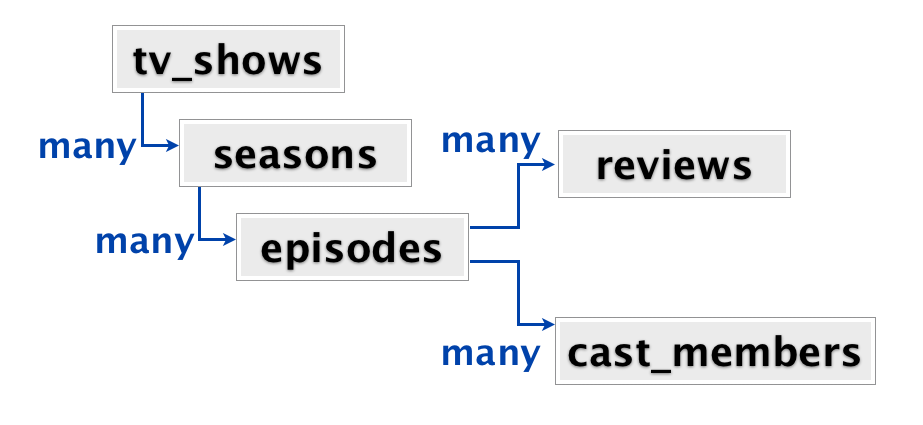
\includegraphics[width=\textwidth]{mongo}
    \caption{Пример структуры документоориентированной БД~\cite{mongo:never}.}
\end{figure}

Графовые БД~--- альтернативный подход к хранению данных в случае, когда важны связи между ними. Такая база состоит из вершин, рёбер и инвариантов графа. Причём рёбра хранят отношения между данными~--- они не вычисляются на лету; каждая вершина представляет собой множество key-value пар, аналогично документу в Document Store~\cite{article:graph}.

Поскольку нам требуется предусмотреть раздельное хранение данных карточек, коллекций карточек и пользователей~(\ref{storage}), документоориентированная модель, где бы условием эффективной работы~\cite{article:join} было хранение всех карточек пользователя в одном документе с его личными данными, не подходит для нашего проекта. Поскольку отношения между сущностями могут изменяться~(\ref{arch}), графовая БД также не удовлетворяет требованиям.

Таким образом, была выбрана NoSQL key-value модель.

Популярные key-value СУБД~--- Amazon DynamoDB, Redis и Aerospike.

DynamoDB на сервере, отличном от Amazon AWS, использует исполняемый .jar файл, то есть работает в виртуальной машине Java; две другие СУБД запускаются непосредственно. Поскольку не планируется развёртывание на Amazon AWS, DynamoDB нам не подходит.

Для добавления нового сервера (node) с целью объединения в кластер в Aerospike достаточно сконфигурировать эту node и присоединение, как и распределение данных, произойдёт автоматически. В Redis для создания кластера необходимо по крайней мере 3 master node, причём он перестанет функционировать в случае обрыва связи хотя бы с одной из них (single point of failure).

\sloppy
По этим причинам в качестве СУБД была выбрана Aerospike Community Edition.

\lstset{style=sharpc}
\begin{lstlisting}
# Aerospike installing:
wget -O aerospike-server.tgz 'https://www.aerospike.com/download/server/latest/artifact/ubuntu20'
tar -xvf aerospike-server.tgz
wget -O aerospike-tools.tgz 'https://www.aerospike.com/download/tools/latest/artifact/ubuntu20'
tar -xvf aerospike-tools.tgz
sudo service aerospike start
sudo vim /etc/aerospike/aerospike.conf
# clean partition before reusing: (inputFile, outputFile)
dd if=/dev/zero of=/dev/destination/disk
\end{lstlisting}

\subsection{Веб-фреймворк}
Из девяти языков программирования, поддерживаемых Aerospike~\cite{aero:clients}, у автора наибольший опыт работы с C\# и Python. Поскольку C\# обеспечивает статическую типизацию, что упрощает поддержку проекта, и является компилируемым, то есть на сервере будет запущен непосредственно исполняемый файл приложения, он был выбран в качестве языка разработки.

\sloppy
.NET Framework поддерживает только ОС Windows, тогда как Aerospike~--- только Linux. Поэтому мы будем использовать .NET Core, обеспечивающий работу .NET в ОС Linux.

В фреймворке .NET Core для разработки web-приложения доступны:
\begin{itemize}
    \item ASP.NET Blazor Server App,
    \item ASP.NET Web API,
    \item ASP.NET Web App.
\end{itemize}
Первый фреймворк предназначен для разработки клиентской части приложения, третий~--- для одновременной разработки backend и frontend. Поскольку цель работы~--- только разработка backend-части, был выбран фреймворк ASP.NET Web API.

\subsection{Интерфейс взаимодействия}
В настоящее время стандартом разработки Web API является подход Representational State Transfer (REST), однако часто используются альтернативные подходы, такие как язык запросов и среда их выполнения GraphQL.

Недостатки API, основанного на REST~\cite{graphql:rest}:
\begin{itemize}
    \item Сервер определяет фиксированный набор запросов, которые может отправлять клиент;
    \item Для получения нескольких объектов потребуется послать несколько запросов.
\end{itemize}
Недостатки API, основанного на GraphQL~\cite{graphql:rest}:
\begin{itemize}
    \item Все запросы клиента отправляются на один адрес (single endpoint), таким образом, невозможно использовать HTTP-кеширование и необходимо реализовать собственное;
    \item Клиентское приложение может запрашивать любой набор данных, предусмотренных оговоренной схемой. Поэтому необходимо разработать схему\footnote{Схема~--- объект, структурно похожий на JSON, перечисляющий и описывающий виды запросов; объекты и их поля, которые могут быть включены в запрос или отправлены на сервер.}, исключающую запросы, выполнение которых негативно скажется на производительности сервера и заблокирует исполнение остальных.
\end{itemize}

Поскольку нам понадобится отправлять клиентскому приложению различные множества флеш-карт и различные наборы данных пользователя (включая коллекции и флеш-карты), для уменьшения числа запросов к API будем использовать технологию GraphQL.

В качестве библиотеки, реализующей GraphQL, выберем HotChocolate ввиду наличия подробной документации и возможности работы ``code-first''~--- автоматической генерации GraphQL-схемы на основе классов C\#.

\section{Проектирование}
Поскольку наше API ориентировано на работу с клиентским приложением, первоначально необходимо определить GraphQL-схему, описав всевозможные запросы.

Нам потребуется получать и отправлять данные пользователя:
\begin{itemize}
    \item Логин,
    \item Hash пароля,
    \item Email,
    \item Его коллекции флеш-карт,
    \item Его флеш-карты.
\end{itemize}
При всяком запросе коллекции необходимо предоставить:
\begin{itemize}
    \item Название,
    \item Описание,
    \item Содержащиеся в ней флеш-карты.
\end{itemize}
Для каждой флеш-карты необходимо предоставить:
\begin{itemize}
    \item Лицевую сторону,
    \item Обратную сторону.
\end{itemize}

Поскольку получение всех коллекций и всех карточек~--- задача ресурсоёмкая и не всегда требуемая (например, при авторизации пользователя или просмотре информации в личном кабинете достаточно первых трёх полей), необходимо также описать запросы, не запускающие эту задачу.

Исходя из этих соображений, была разработана схема запросов, изображенная на Рис.~\ref{fig:schema}. Запрос $hello()$ используется для первоначальной проверки соединения: он всегда выполняется успешно и возвращает ``World!''.

\begin{figure}[ht]
    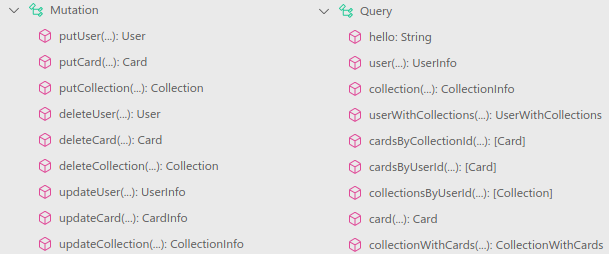
\includegraphics[width=\textwidth]{Schema}
    \caption{GraphQL-схема доступных запросов к API.}
    \label{fig:schema}
\end{figure}

Кроме того, внутри приложения удобно хранить и передавать Id вместо логинов и имён (в случае с коллекциями и карточками это необходимо, поскольку различные пользователи могут создать коллекции с одинаковыми именами). Соответственно, нужно реализовать возможность получения User.Id по его логину User.Login и наоборот~--- это обеспечивает перегруженный метод $user(...): UserInfo$, в качестве аргумента которого может выступать как Id, так и Login.

\subsection{Архитектура} \label{arch}
Будем использовать монолитную архитектуру, поскольку она проще в разработке и развёртывании. Связь с БД будет реализована при помощи отдельных классов; GraphQL-сервер подключим в качестве сервиса.

Предусмотрим возможность будущей реализации совместного использования коллекций, то есть разрешим пользователю назначать других пользователей, которые получат полный доступ к управлению его коллекцией и карточками в ней. Для этого в модели пользователя~(Рис.~\ref{fig:models}) будем хранить только список Id его коллекций. Тогда когда пользователь захочет поделиться коллекцией, нам будет достаточно добавить её Id в список соответствующего получателя. Аналогично, для обеспечения перемещения карточек между коллекциями, в модели коллекции будем хранить список Id принадлежащих ей карточек.

% Без аутентификации это не имеет смысла: клиент получит и может редактировать инфу любого пользователя. При этом также нельзя сказать, что приложение рассчитано на одного пользователя.
% AerospikeClient следовало реализовать в виде DLL с независимыми моделями и без вшивания бизнес-логики, без проверок IsActive: только получи и положи. В текущем положении вещей GraphQL обращается к AerospikeClient напрямую и проверки делаюся частично на стороне Query/Mutation, частично в клиенте базы. Фигня. Остальное-то приложение зачем?

\begin{figure}[ht]
    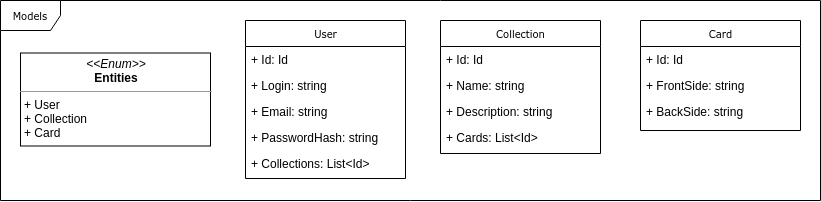
\includegraphics[width=\textwidth]{Models}
    \caption{UML-диаграмма классов используемых моделей.}
    \label{fig:models}
\end{figure}

Разделим работу с БД по назначению: AerospikeManagingClient~(Рис.~\ref{fig:aeroclient}) будет использован единожды, чтобы создать вторичные индексы в базе для обеспечения последующей работы приложения. AerospikeQueryClient используется для получения данных из базы, AerospikeWriteClient~--- для всех операций, изменяющих данные в БД.

\begin{figure}[ht]
    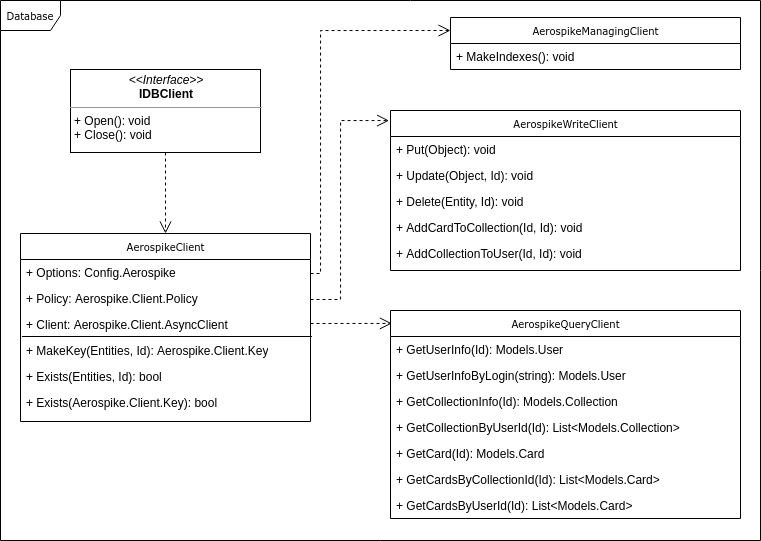
\includegraphics[width=\textwidth]{Database}
    \caption{UML-диаграмма классов работы с БД.}
    \label{fig:aeroclient}
\end{figure}

Так будет организовано взаимодействие клиента, подключённого к нашему API, и серверного приложения. От запроса данных до их получения:

\begin{figure}[ht]
    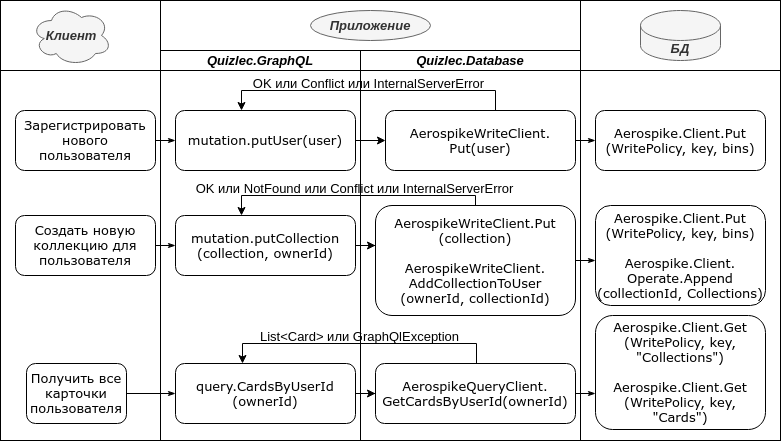
\includegraphics[width=\textwidth]{Sequence}
    \caption{Диаграмма последовательности примеров запросов.}
    \label{fig:sequence}
\end{figure}

\subsection{Схема хранения} \label{storage}
Схема хранения данных в базе будет соответствовать схеме, используемой внутри приложения, с добавлением поля ``IsActive'' типа integer. При работе с C\#-библиотекой integer неявно приводится к bool и обратно, что позволяет использовать это поле как bool внутри приложения. Значение этого поля будет проверяться при каждом запросе к строке: в случае false данные считаются удалёнными. Таким образом, при запросе на удаление данных вместо их фактического удаления из базы мы только помечаем их удалёнными. Это обеспечивает возможность последующего восстановления данных и накопления статистики использования нашего приложения.

Поскольку в Aerospike нет такого понятия как внешний ключ, для сохранения связей между данными рекомендуется~\cite{aero:foreign} использовать списки. Будем использовать списки из Id, как и в самом приложении.

В Aerospike доступны следующие типы данных: integer, double, string, bytes и, соответственно, List<type> и Map<type : type>, где type от каждого из четырёх.
Id реализуем типа integer, что в сравнении с типом string позволит более быстро выполнять запросы по вторичному индексу.

\begin{figure}[ht]
    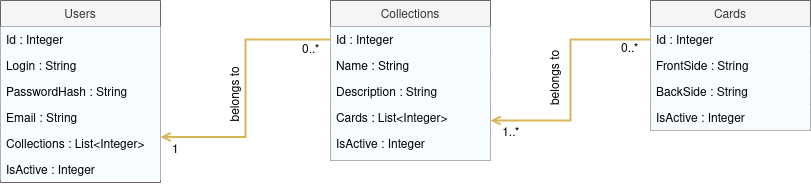
\includegraphics[width=\textwidth]{DB_layout}
    \caption{Диаграмма хранения данных в БД.}
    \label{fig:database}
\end{figure}

\section{Разработка}

\subsection{Реализация запросов}
Каждый запрос выполняется внутри конструкции try-catch, что позволяет продолжать работу приложения даже в случае внутренней ошибки. Кроме того, реализованы пользовательские исключения и их обработчики, благодаря чему API возвращает корректный HTTP-код ошибки с пояснением, что позволяет пользователю локализовать проблему и исправить запрос.
\lstset{style=sharpc}
\begin{lstlisting}
// GraphQL.Query
public UserWithCollections GetUserWithCollections
    (string login)
{
    try
    {
        var client = new AerospikeQueryClient();
        var user = client.GetUserInfoByLogin(login);
        var collections =
            client.GetCollectionsByUserId(user.Id);
        client.Close();
        var res = new UserWithCollections()
        {
            Id = user.Id, Login = user.Login,
            Email = user.Email,
            Collections = collections,
            CollectionsCount = collections.Count
        };
        return res;
    }
    catch (NotFoundException e)
    {
        throw new GraphQlException("User not found. "
        + e.Message, HttpStatusCode.NotFound);
    }
    catch (Exception)
    {
        throw new GraphQlException(
            "Could not get user.",
            HttpStatusCode.InternalServerError);
    }
}
\end{lstlisting}

Обращение к библиотеке работы с БД также использует конструкцию try-catch и передаёт ``наверх'', в том числе в сервис работы с GraphQL, пользовательские исключения, что позволит нам оперативно исправлять возможные ошибки на стороне сервера и скрывать от пользователя технические подробности внутренней работы приложения.

\lstset{style=sharpc}
\begin{lstlisting}
//  Database.AerospikeQueryClient
public User GetUserInfoByLogin(string login)
{
    try
    {
        var res = new List<User>();
        var stmt = new Statement();
        stmt.SetNamespace(Options.Namespace);
        stmt.SetSetName(Options.Set.User);
        stmt.SetBinNames("Id", "Login",
            "PasswordHash", "Email", "IsActive");
        stmt.Filter = Filter.Equal("Login", login);
        RecordSet rs = Client.Query(
            (QueryPolicy) Policy, stmt);
        while (rs.Next())
        {
            var r = rs.Record;
            if (r.GetBool("IsActive"))
                res.Add(new User()
                {
                    Id = r.GetInt("Id"),
                    Login = login,
                    Email = r.GetString("Email"),
                });
        }
        rs.Dispose();
        if (res.Count == 1)
            return res[0];
        if (res.Count == 0)
            throw new UserNotFoundException
                ($"The user with login={login}
                    doesn't exist.");
        if (res.Count > 1)
            throw new DatabaseQueryException
                ($"Too many users with
                    login={login}: {res.Count}.");
        else
            throw new DatabaseQueryException();
    }
    catch (AerospikeException e)
    {
        throw new DatabaseQueryException
            ("Please create User:Login index
                first.", e);
    }
    catch (Exception e)
    {
        throw new DatabaseQueryException(
            "Cannot get user by login", e);
    }
}
\end{lstlisting}

Полный код проекта можно найти на странице \url{https://github.com/studokim/Quizlec/}.

\section*{Заключение}
В процессе разработки были достигнуты следующие результаты:
\begin{itemize}
    \item Выбраны, изучены и использованы технологии работы с базой данных, разработки серверного приложения и его взаимодействия с клиентским приложением;
    \item Разработана архитектура приложения
    \item Разработана схема хранения данных;
    \item Реализованы типичные запросы к данным;
    \item Создан работоспособный API.
\end{itemize}
\setmonofont[Mapping=tex-text]{CMU Typewriter Text}
\bibliographystyle{ugost2008ls}
\bibliography{diploma.bib}
\end{document}
